\documentclass[11pt,letterpaper]{article}
\usepackage[utf8]{inputenc}

%----- Configuración del estilo del documento------%
\usepackage{epsfig,graphicx}
\usepackage[left=2cm,right=2cm,top=1.8cm,bottom=2.3cm]{geometry}
\usepackage{fancyhdr}
\usepackage{lastpage}

\usepackage{xcolor}
\usepackage{soul}
\newcommand{\mathcolorbox}[2]{\colorbox{#1}{$\displaystyle #2$}}

%Color bibi
\definecolor{bibi}{RGB}{0,103,148}
% Otros colores

%------ Paquetes de dibujo --------%
\usepackage{tikz}
\usepackage{circuitikz}

%------ Paquetes para mantener las imágenes en su lugar --------%
\usepackage{float}


\usepackage{cite}
\usepackage{multicol}
\setlength{\columnsep}{1.5cm}
\setlength{\columnseprule}{.5pt}

\pagestyle{fancy}
\fancyhf{}
\rfoot{\textit{Página \thepage \hspace{1pt} de \pageref{LastPage}}}

%------ Paquetes matemáticos básicos --------%
\usepackage{amsmath}
\usepackage{amssymb}
\usepackage{amsthm}

\begin{document}
%------ Encabezado -------- %
\begin{center}
    \begin{minipage}{3cm}
    	\begin{center}
    		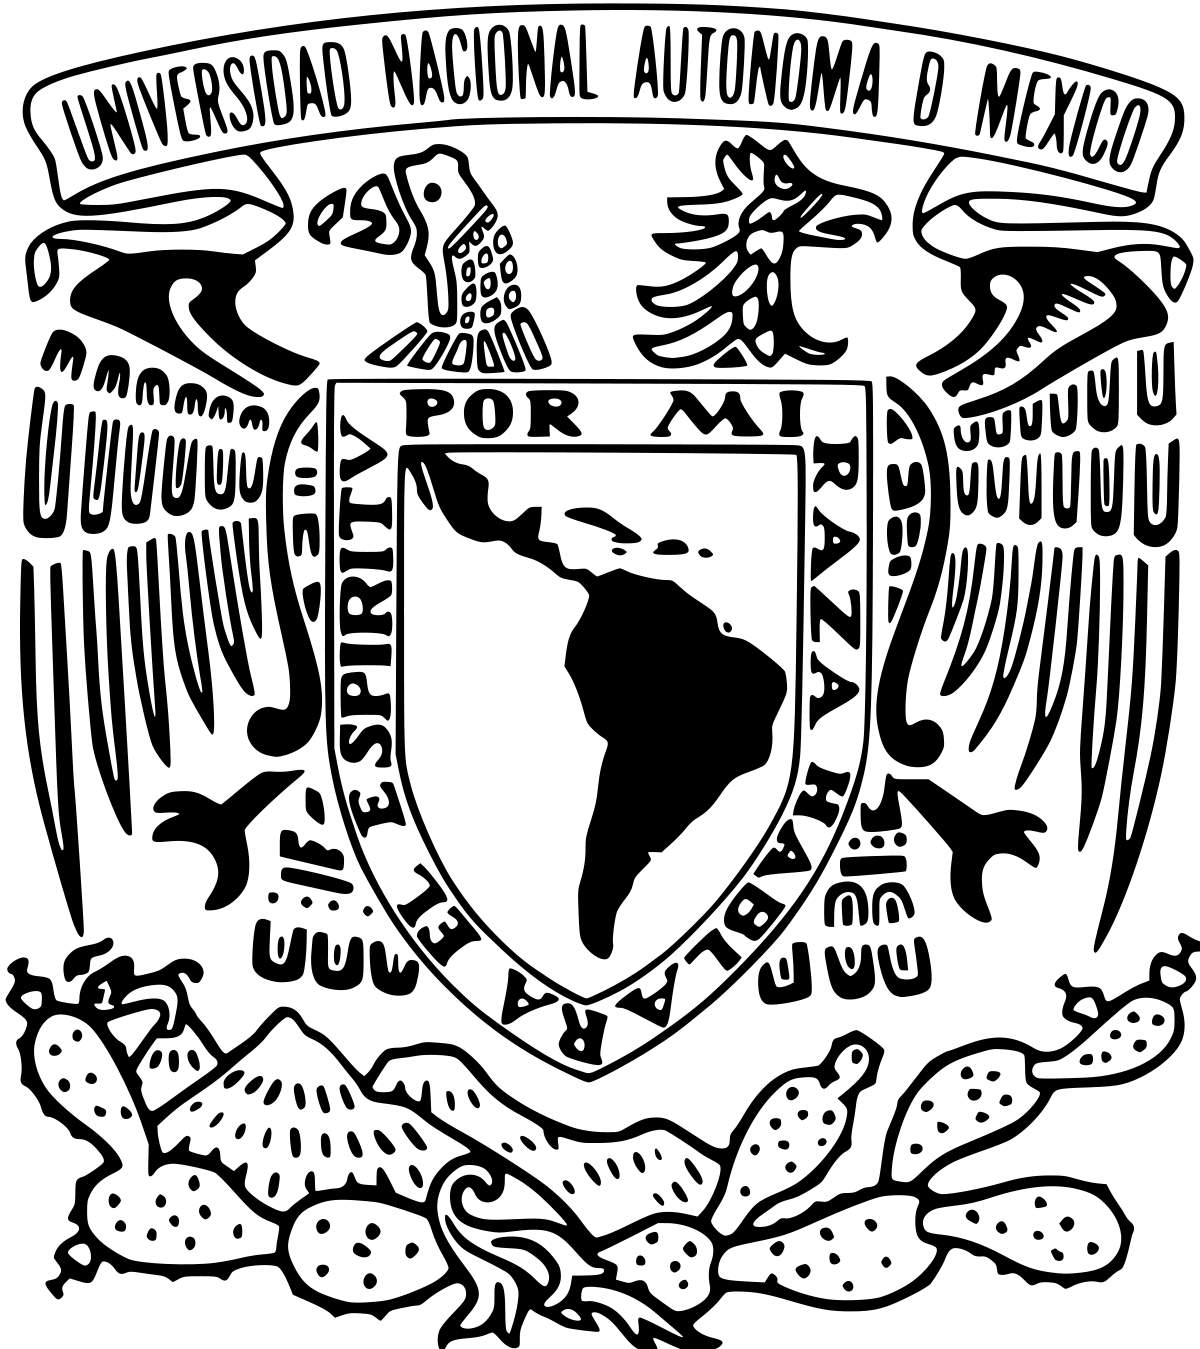
\includegraphics[height=3.3cm]{src/Img/Logo_UNAM.png}
    	\end{center}
    \end{minipage}\hfill
    \begin{minipage}{10cm}
    	\begin{center}
    	\textbf{\large Universidad Nacional Autónoma de México}\\[0.1cm]
        \textbf{Facultad de Ciencias}\\[0.1cm]
        \textbf{Análisis de Algoritmos  $|$ 7083}\\[0.1cm]
        Tarea 3 : $|$ Programacion Dinamica\\[0.1cm]
        Sosa Romo Juan Mario $|$ 320051926 \\[0.1cm]
        25/09/24
    	\end{center}
    \end{minipage}\hfill
    \begin{minipage}{3cm}
    	\begin{center}
    		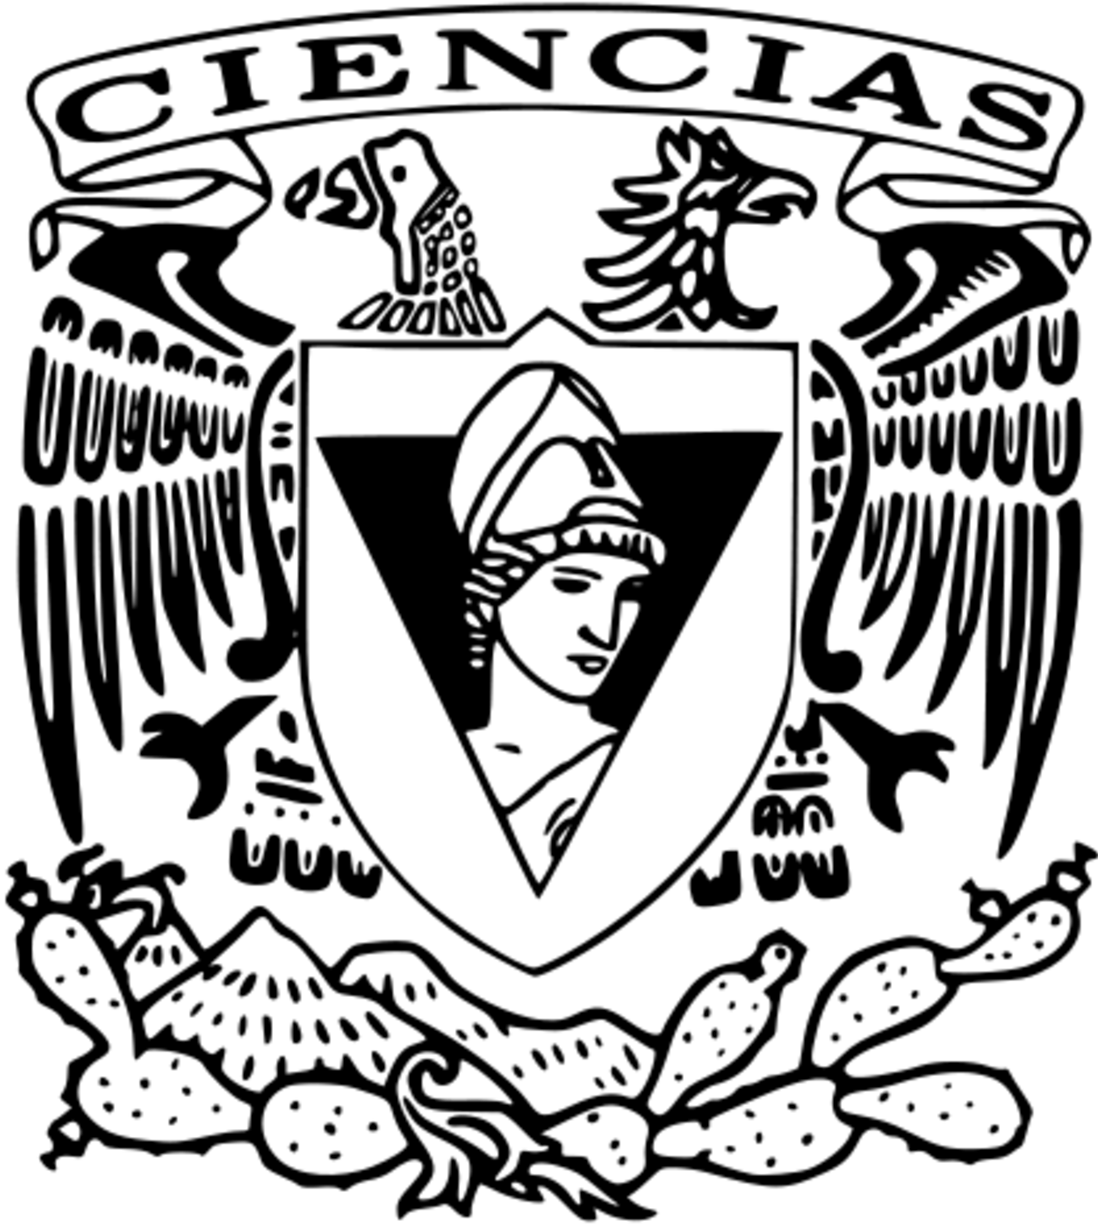
\includegraphics[height=3.3cm]{src/Img/Logo_FC.png}
    	\end{center}
    \end{minipage}
\end{center}


\rule{16.99cm}{0.1mm}

%------ Ejercicios -------- %
\begin{enumerate}
    \item \textbf{Basado en las notas del curso, por favor calcula el protocolo de
teletransportación cuántica usando el estado de Bell $\ket{\beta}_{02}$}\vspace{.2cm}

\[
    \ket{\beta_{02}} = \displaystyle\frac{\ket{01}+\ket{10}}{\sqrt{2}}  
\]

\textbf{Y el estado $\ket{psi}$ a ser teletransportado definido como:}
\[
    \ket{\psi} = \alpha \ket{0} + \beta{1}  
\]

\textbf{Puedes basarte de la fig1 para seguir visualmente el protocolo.}
 
\begin{center}
    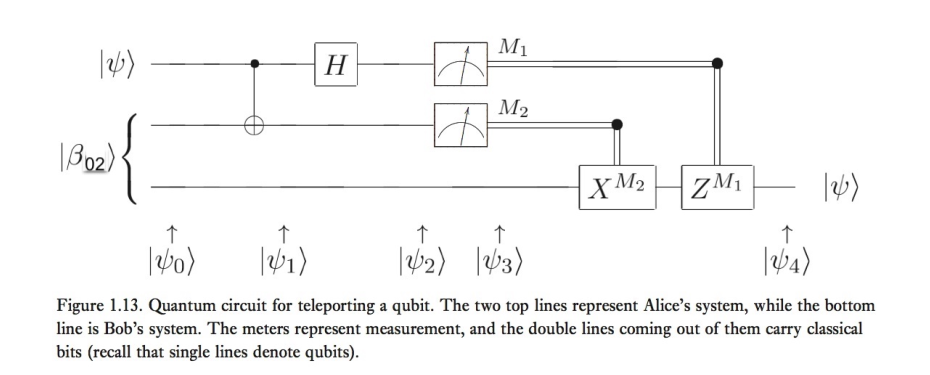
\includegraphics[height=6cm]{src/Img/1.png}
\end{center}

\end{enumerate}

% \textbf{}\vspace{.2cm}
% \textcolor{bibi}{}
% \begin{quote}
% \end{quote}

\end{document}
